\documentclass[a4paper,11pt]{article}

% === PACKAGES ===
\usepackage[utf8]{inputenc}
\usepackage[T1]{fontenc}
\usepackage[french]{babel}
\usepackage{amsmath,amssymb,amsthm}
\usepackage{graphicx}
\usepackage{booktabs}
\usepackage{geometry}
\usepackage{hyperref}
\usepackage{caption}
\usepackage{subcaption}
\usepackage{float}
\usepackage{enumitem}

\geometry{margin=2.5cm}

% === CHIFFRES AUTO-GENERES (source unique de verite) ===
% Tous les chiffres numeriques des tables (Delta/Gamma/Vega/Euler/EDP)
% sont injectes via \newcommand depuis ../_audit/numbers.tex,
% lui-meme regenere par .venv-audit/bin/python ../_audit/extract_numbers.py.
% Auto-generated by _audit/extract_numbers.py - DO NOT EDIT MANUALLY
% Source unique de verite pour rapport_latex/rapport.tex.
% Regenerer via: .venv-audit/bin/python _audit/extract_numbers.py
%
% Convention statistique : 'Ecart-type' designe l'erreur standard
% SE = sigma_sample / sqrt(N) (= IC95 / 1.96). 'IC 95%' = +/-1.96 * SE.
% Pour FD, IC obtenu par bootstrap 200 replicas (notebook cell 7).

\newcommand{\paramN}{50\,000}
\newcommand{\bsPrice}{10.4506}
\newcommand{\bsDelta}{0.6368}
\newcommand{\bsGamma}{0.0188}
\newcommand{\bsVega}{37.52}
\newcommand{\bsGammaFive}{0.01876}
\newcommand{\bsVegaThree}{37.524}
\newcommand{\deltaFdEst}{0.6378}
\newcommand{\deltaPwEst}{0.6379}
\newcommand{\deltaMalEst}{0.6404}
\newcommand{\deltaFdSe}{0.0006}
\newcommand{\deltaPwSe}{0.0006}
\newcommand{\deltaMalSe}{0.0042}
\newcommand{\deltaFdIc}{0.0012}
\newcommand{\deltaPwIc}{0.0013}
\newcommand{\deltaMalIc}{0.0083}
\newcommand{\deltaFdErrPct}{0.15}
\newcommand{\deltaPwErrPct}{0.16}
\newcommand{\deltaMalErrPct}{0.56}
\newcommand{\deltaRatioMalPw}{6.5}
\newcommand{\deltaVarRatioMalPw}{43}
\newcommand{\gammaFdEst}{0.01828}
\newcommand{\gammaMalEst}{0.01923}
\newcommand{\gammaFdSe}{0.00034}
\newcommand{\gammaMalSe}{0.00045}
\newcommand{\gammaFdIc}{0.00066}
\newcommand{\gammaMalIc}{0.00088}
\newcommand{\gammaFdErrPct}{2.57}
\newcommand{\gammaMalErrPct}{2.47}
\newcommand{\vegaFdEst}{37.61}
\newcommand{\vegaPwEst}{37.61}
\newcommand{\vegaMalEst}{38.45}
\newcommand{\vegaFdSe}{0.20}
\newcommand{\vegaPwSe}{0.21}
\newcommand{\vegaMalSe}{0.90}
\newcommand{\vegaFdIc}{0.39}
\newcommand{\vegaPwIc}{0.41}
\newcommand{\vegaMalIc}{1.76}
\newcommand{\vegaFdErrPct}{0.23}
\newcommand{\vegaPwErrPct}{0.24}
\newcommand{\vegaMalErrPct}{2.47}
\newcommand{\vegaRatioMalPw}{4.3}
\newcommand{\vegaVarRatioMalPw}{18}
\newcommand{\varRatioFdPw}{0.84}
\newcommand{\varRatioPwPw}{1}
\newcommand{\varRatioMalPw}{43}
\newcommand{\eulerErrTen}{0.0033}
\newcommand{\eulerErrFifty}{0.0002}
\newcommand{\eulerErrHundred}{0.0001}
\newcommand{\eulerErrFiveHundred}{0.0006}
\newcommand{\pdePrice}{10.4491}
\newcommand{\pdeDelta}{0.6175}
\newcommand{\pdeGamma}{0.0193}
\newcommand{\pdeVega}{37.47}
\newcommand{\pdeErrPrice}{0.0014}
\newcommand{\pdeErrDelta}{0.0193}
\newcommand{\pdeErrGamma}{0.0005}
\newcommand{\pdeErrVega}{0.06}


% === THEOREMES ===
\theoremstyle{definition}
\newtheorem{definition}{Définition}[section]
\newtheorem{propriete}{Propriété}[section]
\newtheorem{theoreme}{Théorème}[section]
\newtheorem{remarque}{Remarque}[section]

% === TITRE ===
\title{\textbf{Monte Carlo Computation of Sensitivities}\\[0.5cm]
\large Étude Comparative des Approches Numériques pour le Calcul des Greeks}
\author{Dan Allouche\\[0.3cm]
\textit{Master MASEF}\\
\textit{Université Paris-Dauphine}}
\date{\today}

\begin{document}

\maketitle

\begin{abstract}
Ce rapport présente une étude approfondie des différentes méthodes de calcul des sensibilités (Greeks) d'options européennes par simulation Monte Carlo. Nous développons et comparons trois approches fondamentales : les différences finies, la méthode pathwise (différentiation automatique adjointe), et le calcul de Malliavin (likelihood ratio method). Chaque méthode est analysée théoriquement puis validée numériquement par rapport aux formules analytiques de Black-Scholes. Nous étudions également l'impact de la discrétisation temporelle (schéma d'Euler) et proposons une validation croisée avec une approche par équations aux dérivées partielles (EDP). Les recommandations pratiques sont formulées en fonction du contexte d'application.
\end{abstract}

\tableofcontents
\newpage

% ============================================
\section{Introduction}
% ============================================

\subsection{Contexte et Motivation}

Le calcul des sensibilités, communément appelées \textbf{Greeks} en référence aux lettres grecques utilisées pour les noter, constitue un pilier fondamental de la finance quantitative moderne. Ces quantités mesurent la sensibilité du prix d'un instrument dérivé aux variations de ses paramètres sous-jacents.

\subsubsection{Importance des Greeks en Pratique}

Les Greeks sont essentiels pour plusieurs raisons :

\begin{enumerate}[label=(\roman*)]
    \item \textbf{Gestion des risques (hedging)} : Le Delta permet de construire un portefeuille neutre (delta-hedging), le Gamma mesure la vitesse de réajustement nécessaire, et le Vega quantifie l'exposition à la volatilité implicite.
    
    \item \textbf{Valorisation et P\&L} : L'expansion de Taylor du prix d'une option utilise directement les Greeks :
    $$\Delta C \approx \Delta \cdot \Delta S + \frac{1}{2}\Gamma \cdot (\Delta S)^2 + \mathcal{V} \cdot \Delta\sigma + \Theta \cdot \Delta t$$
    
    \item \textbf{Réglementation} : Les cadres réglementaires (Bâle III/IV) exigent le calcul des sensibilités pour le calcul des charges en capital.
    
    \item \textbf{Trading} : Les market-makers utilisent les Greeks pour ajuster leurs cotations et gérer leur inventaire.
\end{enumerate}

\subsubsection{Pourquoi Monte Carlo ?}

Pour les options européennes simples, les formules analytiques de Black-Scholes fournissent les Greeks de manière exacte. Cependant, pour de nombreux produits complexes, aucune formule fermée n'existe :

\begin{itemize}
    \item Options asiatiques (payoff dépendant de la moyenne du sous-jacent)
    \item Options barrières (activation/désactivation conditionnelle)
    \item Options sur panier (plusieurs sous-jacents)
    \item Options sous modèles à volatilité stochastique (Heston, SABR)
\end{itemize}

Dans ces cas, la simulation Monte Carlo devient l'outil privilégié, d'où l'importance de maîtriser les techniques de calcul des Greeks par simulation.

\subsection{Objectifs du Projet}

Ce rapport poursuit les objectifs suivants :

\begin{enumerate}
    \item \textbf{Développer théoriquement} trois méthodes de calcul des Greeks par Monte Carlo
    \item \textbf{Implémenter et comparer} ces méthodes sur un cas test (call européen Black-Scholes)
    \item \textbf{Analyser} les propriétés statistiques des estimateurs (biais, variance, convergence)
    \item \textbf{Étudier l'impact} de la discrétisation temporelle (Euler vs Exact)
    \item \textbf{Valider} les résultats par une approche EDP indépendante
    \item \textbf{Formuler des recommandations} pratiques selon le contexte d'utilisation
\end{enumerate}

\subsection{Organisation du Rapport}

\begin{table}[H]
\centering
\begin{tabular}{cl}
\toprule
\textbf{Section} & \textbf{Contenu} \\
\midrule
\S 2 & Cadre théorique : modèle de Black-Scholes et définitions \\
\S 3 & Méthode des Différences Finies \\
\S 4 & Méthode Pathwise (Différentiation Automatique) \\
\S 5 & Méthode de Malliavin (Likelihood Ratio) \\
\S 6 & Résultats numériques pour Delta, Gamma et Vega \\
\S 7 & Impact de la discrétisation Euler \\
\S 8 & Validation par approche EDP \\
\S 9 & Conclusion et recommandations \\
\bottomrule
\end{tabular}
\caption{Plan du rapport}
\end{table}

% ============================================
\section{Cadre Théorique}
% ============================================

\subsection{Le Modèle de Black-Scholes-Merton}

\subsubsection{Dynamique du Sous-jacent}

Nous considérons le modèle standard de Black-Scholes-Merton (1973) pour la dynamique du prix d'un actif risqué.

\begin{definition}[Modèle de Black-Scholes]
Sous la mesure risque-neutre $\mathbb{Q}$, le prix du sous-jacent $S_t$ suit l'équation différentielle stochastique :
$$dS_t = r S_t \, dt + \sigma S_t \, dW_t$$
où :
\begin{itemize}
    \item $r$ : taux d'intérêt sans risque (constant)
    \item $\sigma$ : volatilité (constante)
    \item $W_t$ : mouvement brownien standard sous $\mathbb{Q}$
\end{itemize}
\end{definition}

\subsubsection{Solution Exacte}

L'EDS ci-dessus admet une solution explicite (formule de géométrie brownienne) :

\begin{propriete}[Solution de l'EDS de Black-Scholes]
Pour tout $T > 0$, le prix terminal s'écrit :
$$S_T = S_0 \exp\left(\left(r - \frac{\sigma^2}{2}\right)T + \sigma W_T\right)$$

De manière équivalente, en introduisant $Z \sim \mathcal{N}(0,1)$ :
$$S_T = S_0 \exp\left(\left(r - \frac{\sigma^2}{2}\right)T + \sigma \sqrt{T} Z\right)$$
\end{propriete}

Cette formule permet une simulation exacte de $S_T$ sans discrétisation temporelle.

\subsection{Options Européennes et Greeks}

\subsubsection{Payoff et Valorisation}

\begin{definition}[Call Européen]
Un call européen de strike $K$ et maturité $T$ donne le droit (non l'obligation) d'acheter l'actif sous-jacent au prix $K$ à la date $T$. Son payoff est :
$$g(S_T) = (S_T - K)^+ = \max(S_T - K, 0)$$
\end{definition}

Par absence d'opportunité d'arbitrage, le prix du call à la date $t=0$ est :
$$C(S_0, K, T, r, \sigma) = e^{-rT} \mathbb{E}^{\mathbb{Q}}[g(S_T)]$$

\subsubsection{Formule de Black-Scholes}

\begin{theoreme}[Formule de Black-Scholes pour un Call]
Le prix d'un call européen est donné par :
$$C = S_0 \Phi(d_1) - K e^{-rT} \Phi(d_2)$$
où :
$$d_1 = \frac{\ln(S_0/K) + (r + \sigma^2/2)T}{\sigma\sqrt{T}}, \quad d_2 = d_1 - \sigma\sqrt{T}$$
et $\Phi$ désigne la fonction de répartition de la loi normale standard.
\end{theoreme}

\subsubsection{Définition des Greeks}

\begin{definition}[Greeks étudiés]
Les sensibilités du premier et second ordre considérées sont :

\begin{align}
\Delta &= \frac{\partial C}{\partial S_0} & \text{(sensibilité au prix spot)} \\[0.3cm]
\Gamma &= \frac{\partial^2 C}{\partial S_0^2} & \text{(convexité / sensibilité du Delta)} \\[0.3cm]
\mathcal{V} &= \frac{\partial C}{\partial \sigma} & \text{(sensibilité à la volatilité)}
\end{align}
\end{definition}

\subsubsection{Formules Analytiques des Greeks}

Par dérivation de la formule de Black-Scholes :

\begin{propriete}[Greeks analytiques]
\begin{align}
\Delta &= \Phi(d_1) \\
\Gamma &= \frac{\phi(d_1)}{S_0 \sigma \sqrt{T}} \\
\mathcal{V} &= S_0 \phi(d_1) \sqrt{T}
\end{align}
où $\phi(x) = \frac{1}{\sqrt{2\pi}} e^{-x^2/2}$ est la densité de la loi normale standard.
\end{propriete}

Ces formules serviront de \textbf{benchmark} pour valider nos estimateurs Monte Carlo.

\subsection{Régularité du Payoff et Conséquences}

La régularité du payoff $g$ joue un rôle crucial dans le choix de la méthode de calcul des Greeks.

\begin{propriete}[Régularité du payoff call]
Pour $g(S) = (S-K)^+$ :
\begin{enumerate}
    \item $g$ est Lipschitz : $|g(S_1) - g(S_2)| \leq |S_1 - S_2|$
    \item $g'(S) = \mathbb{1}_{S > K}$ presque partout
    \item $g''(S) = \delta_K(S)$ (distribution de Dirac au point $K$)
\end{enumerate}
\end{propriete}

\begin{remarque}
La discontinuité de $g'$ en $S=K$ n'est pas problématique car $\mathbb{P}(S_T = K) = 0$ (le brownien ne charge pas les points). En revanche, la singularité de $g''$ rend la méthode Pathwise inapplicable pour le Gamma.
\end{remarque}

\subsection{Paramètres de Simulation}

Pour tous les tests numériques, nous utilisons les paramètres standard suivants :

\begin{table}[H]
\centering
\begin{tabular}{lcc}
\toprule
\textbf{Paramètre} & \textbf{Notation} & \textbf{Valeur} \\
\midrule
Prix spot initial & $S_0$ & 100 \\
Strike & $K$ & 100 (ATM) \\
Maturité & $T$ & 1 an \\
Taux sans risque & $r$ & 5\% \\
Volatilité & $\sigma$ & 20\% \\
Nombre de simulations & $N$ & 50 000 \\
\bottomrule
\end{tabular}
\caption{Paramètres de référence}
\end{table}

Avec ces paramètres, les valeurs théoriques de Black-Scholes sont :
$$\text{Prix} = \bsPrice, \quad \Delta = \bsDelta, \quad \Gamma = \bsGamma, \quad \mathcal{V} = \bsVega$$

% ============================================
\section{Méthode des Différences Finies}
% ============================================

\subsection{Principe Général}

La méthode des différences finies est l'approche la plus intuitive : elle approxime la dérivée par un quotient différentiel.

\begin{definition}[Estimateur FD]
Pour estimer $\frac{\partial C}{\partial \theta}$ où $\theta$ est un paramètre du modèle :
$$\hat{\Delta}_{\text{FD}} = \frac{\hat{C}(\theta + \varepsilon) - \hat{C}(\theta - \varepsilon)}{2\varepsilon}$$
où $\hat{C}(\theta)$ désigne l'estimateur Monte Carlo du prix avec paramètre $\theta$.
\end{definition}

\subsubsection{Application au Delta}

Pour le Delta ($\theta = S_0$) :
$$\hat{\Delta}_{\text{FD}} = \frac{1}{2\varepsilon} \left[ \frac{1}{N}\sum_{i=1}^N e^{-rT} g\left(S_T^{(i)}(S_0 + \varepsilon)\right) - \frac{1}{N}\sum_{i=1}^N e^{-rT} g\left(S_T^{(i)}(S_0 - \varepsilon)\right) \right]$$

\begin{remarque}[Common Random Numbers - CRN]
Pour réduire la variance, il est crucial d'utiliser les \textbf{mêmes tirages aléatoires} $Z^{(i)}$ pour les deux prix $S_0 + \varepsilon$ et $S_0 - \varepsilon$. Cette technique de réduction de variance est appelée "Common Random Numbers".
\end{remarque}

\subsection{Analyse du Biais et de la Variance}

L'estimateur FD présente un compromis biais-variance lié au choix de $\varepsilon$ :

\subsubsection{Biais}

Par développement de Taylor :
$$\frac{C(\theta + \varepsilon) - C(\theta - \varepsilon)}{2\varepsilon} = C'(\theta) + \frac{\varepsilon^2}{6} C'''(\theta) + O(\varepsilon^4)$$

Le biais est donc $O(\varepsilon^2)$ : plus $\varepsilon$ est petit, plus le biais est faible.

\subsubsection{Variance}

La variance de l'estimateur est proportionnelle à $\frac{1}{N\varepsilon^2}$ :
$$\text{Var}(\hat{\Delta}_{\text{FD}}) \approx \frac{1}{N\varepsilon^2} \cdot \text{Var}(g(S_T^+) - g(S_T^-))$$

Plus $\varepsilon$ est petit, plus la variance est élevée.

\subsubsection{Choix Optimal de $\varepsilon$}

L'erreur quadratique moyenne (MSE) s'écrit :
$$\text{MSE} = \text{Biais}^2 + \text{Variance} \propto \varepsilon^4 + \frac{1}{N\varepsilon^2}$$

En minimisant, on obtient :
$$\varepsilon^* \propto N^{-1/6}$$

Pour $N = 50\,000$, une valeur empirique de $\varepsilon \approx 1$ est généralement recommandée.

\subsection{Application au Gamma}

Le Gamma est estimé par différences finies d'ordre 2 :
$$\hat{\Gamma}_{\text{FD}} = \frac{\hat{C}(S_0 + \varepsilon) - 2\hat{C}(S_0) + \hat{C}(S_0 - \varepsilon)}{\varepsilon^2}$$

Cette formule nécessite trois évaluations Monte Carlo avec les mêmes tirages aléatoires.

\subsection{Avantages et Inconvénients}

\begin{table}[H]
\centering
\begin{tabular}{p{6cm}p{6cm}}
\toprule
\textbf{Avantages} & \textbf{Inconvénients} \\
\midrule
\begin{itemize}[leftmargin=*]
    \item Universellement applicable
    \item Simple à implémenter
    \item Fonctionne pour tout payoff
\end{itemize}
&
\begin{itemize}[leftmargin=*]
    \item Compromis biais-variance sur $\varepsilon$
    \item Nécessite 2-3 simulations par Greek
    \item Moins efficace que Pathwise quand applicable
\end{itemize}
\\
\bottomrule
\end{tabular}
\end{table}

% ============================================
\section{Méthode Pathwise (Différentiation)}
% ============================================

\subsection{Principe Fondamental}

La méthode Pathwise, également appelée IPA (Infinitesimal Perturbation Analysis), consiste à \textbf{différentier à l'intérieur de l'espérance} en utilisant la règle de dérivation composée.

\begin{theoreme}[Estimateur Pathwise]
Sous certaines conditions de régularité, on peut écrire :
$$\frac{\partial}{\partial \theta} \mathbb{E}[g(S_T(\theta))] = \mathbb{E}\left[ g'(S_T(\theta)) \frac{\partial S_T}{\partial \theta} \right]$$

L'estimateur Pathwise est alors :
$$\hat{\Delta}_{\text{PW}} = \frac{1}{N} \sum_{i=1}^N e^{-rT} g'(S_T^{(i)}) \frac{\partial S_T^{(i)}}{\partial \theta}$$
\end{theoreme}

\subsection{Calcul des Dérivées pour Black-Scholes}

\subsubsection{Dérivée par rapport à $S_0$ (Delta)}

Partant de $S_T = S_0 \exp\left((r - \frac{\sigma^2}{2})T + \sigma\sqrt{T} Z\right)$ :
$$\frac{\partial S_T}{\partial S_0} = \exp\left(\left(r - \frac{\sigma^2}{2}\right)T + \sigma\sqrt{T} Z\right) = \frac{S_T}{S_0}$$

Pour un call, $g'(S_T) = \mathbb{1}_{S_T > K}$, donc :
$$\hat{\Delta}_{\text{PW}} = \frac{1}{N} \sum_{i=1}^N e^{-rT} \mathbb{1}_{S_T^{(i)} > K} \cdot \frac{S_T^{(i)}}{S_0}$$

\subsubsection{Dérivée par rapport à $\sigma$ (Vega)}

$$\frac{\partial S_T}{\partial \sigma} = S_T \left( -\sigma T + \sqrt{T} Z \right)$$

L'estimateur Pathwise pour Vega est :
$$\hat{\mathcal{V}}_{\text{PW}} = \frac{1}{N} \sum_{i=1}^N e^{-rT} \mathbb{1}_{S_T^{(i)} > K} \cdot S_T^{(i)} \left( -\sigma T + \sqrt{T} Z^{(i)} \right)$$

\subsubsection{Cas du Gamma : Inapplicabilité}

Pour le Gamma, on aurait besoin de $g''(S_T)$. Or :
$$g''(S) = \delta_K(S)$$
où $\delta_K$ est la distribution de Dirac au point $K$. Cette singularité rend l'espérance $\mathbb{E}[g''(S_T) \cdot (\ldots)]$ \textbf{non définie} au sens classique.

\begin{remarque}
L'impossibilité de Pathwise pour Gamma est une limitation fondamentale liée à la non-différentiabilité du payoff call en $K$.
\end{remarque}

\subsection{Conditions d'Applicabilité}

\begin{propriete}[Conditions pour Pathwise]
La méthode Pathwise est applicable si :
\begin{enumerate}
    \item Le payoff $g$ est Lipschitz (ou plus généralement presque partout différentiable)
    \item $\mathbb{E}[|g'(S_T)| \cdot |\partial S_T / \partial \theta|] < \infty$
    \item Les conditions de dominance pour l'échange dérivée-espérance sont satisfaites
\end{enumerate}
\end{propriete}

\subsection{Propriétés Statistiques}

\begin{propriete}[Non-biais et variance]
L'estimateur Pathwise est :
\begin{enumerate}
    \item \textbf{Non biaisé} : $\mathbb{E}[\hat{\Delta}_{\text{PW}}] = \Delta$
    \item \textbf{Variance minimale} parmi les estimateurs étudiés (pour payoffs réguliers)
\end{enumerate}
\end{propriete}

% ============================================
\section{Méthode de Malliavin (LRM)}
% ============================================

\subsection{Idée Fondamentale}

La méthode de Malliavin, aussi appelée Likelihood Ratio Method (LRM) ou Score Function Method, utilise une astuce élégante : au lieu de différentier le payoff, on \textbf{différentie la densité de probabilité}.

\begin{theoreme}[Formule de Malliavin]
Pour $S_T$ de densité $p_\theta(S)$ dépendant du paramètre $\theta$ :
$$\frac{\partial}{\partial \theta} \mathbb{E}[g(S_T)] = \mathbb{E}\left[ g(S_T) \cdot \frac{\partial}{\partial \theta} \ln p_\theta(S_T) \right]$$
\end{theoreme}

\textbf{Avantage majeur} : Le payoff $g$ n'est pas différentié ! La méthode fonctionne donc même pour des payoffs \textbf{discontinus} (options digitales, barrières, etc.).

\subsection{Calcul du Score pour Black-Scholes}

\subsubsection{Score pour Delta}

Sous Black-Scholes, $S_T = S_0 e^{(r-\sigma^2/2)T + \sigma\sqrt{T} Z}$ avec $Z \sim \mathcal{N}(0,1)$.

On peut montrer que le "poids de Malliavin" pour le Delta est :
$$\frac{\partial}{\partial S_0} \ln p(S_T) = \frac{W_T}{S_0 \sigma T} = \frac{Z}{S_0 \sigma \sqrt{T}}$$

L'estimateur Malliavin pour Delta est donc :
$$\hat{\Delta}_{\text{MAL}} = \frac{1}{N} \sum_{i=1}^N e^{-rT} g(S_T^{(i)}) \cdot \frac{Z^{(i)}}{S_0 \sigma \sqrt{T}}$$

\subsubsection{Score pour Gamma}

Pour le Gamma (dérivée seconde), le poids de Malliavin devient :
$$\hat{\Gamma}_{\text{MAL}} = \frac{1}{N} \sum_{i=1}^N e^{-rT} g(S_T^{(i)}) \cdot \frac{(Z^{(i)})^2 - 1}{S_0^2 \sigma^2 T}$$

\subsubsection{Score pour Vega}

$$\hat{\mathcal{V}}_{\text{MAL}} = \frac{1}{N} \sum_{i=1}^N e^{-rT} g(S_T^{(i)}) \cdot \frac{(Z^{(i)})^2 - 1}{\sigma}$$

\subsection{Variance de l'Estimateur Malliavin}

Le principal inconvénient de la méthode de Malliavin est sa \textbf{variance élevée}.

\begin{propriete}[Variance de Malliavin]
La variance de l'estimateur Malliavin est généralement bien supérieure à celle de Pathwise :
$$\text{Var}(\hat{\Delta}_{\text{MAL}}) \gg \text{Var}(\hat{\Delta}_{\text{PW}})$$

Typiquement, $\text{Var}(\hat{\Delta}_{\text{MAL}}) \approx 20-50 \times \text{Var}(\hat{\Delta}_{\text{PW}})$ pour un call ATM.
\end{propriete}

Cette variance élevée provient du poids $Z/(S_0\sigma\sqrt{T})$ qui fluctue fortement.

\subsection{Techniques de Réduction de Variance}

Plusieurs techniques peuvent réduire la variance de Malliavin :
\begin{enumerate}
    \item \textbf{Variables antithétiques} : Utiliser $(Z, -Z)$ simultanément
    \item \textbf{Variables de contrôle} : Utiliser le prix de l'option comme contrôle
    \item \textbf{Formules conditionnelles} : Conditionner sur certaines variables
\end{enumerate}

% ============================================
\section{Résultats Numériques}
% ============================================

\subsection{Comparaison pour Delta}

\begin{figure}[H]
\centering
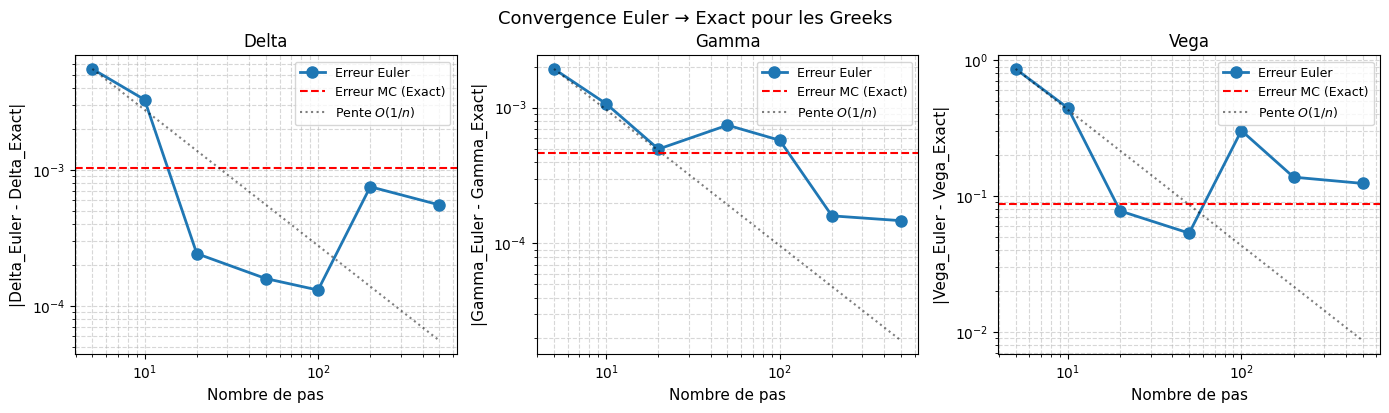
\includegraphics[width=0.95\textwidth]{figures/delta_comparaison.png}
\caption{Comparaison des trois méthodes pour le calcul du Delta. Chaque barre représente l'estimation Monte Carlo avec son intervalle de confiance à 95\%. La ligne horizontale rouge indique la valeur théorique de Black-Scholes ($\Delta = \bsDelta$).}
\label{fig:delta}
\end{figure}

\subsubsection{Analyse des Résultats Delta}

\begin{table}[H]
\centering
\begin{tabular}{lcccc}
\toprule
\textbf{Méthode} & \textbf{Estimation} & \textbf{SE} & \textbf{IC 95\%} & \textbf{Erreur rel.} \\
\midrule
Black-Scholes (ref.) & \bsDelta & -- & -- & -- \\
Différences Finies & \deltaFdEst & \deltaFdSe & $\pm \deltaFdIc$ & \deltaFdErrPct\% \\
Pathwise & \deltaPwEst & \deltaPwSe & $\pm \deltaPwIc$ & \deltaPwErrPct\% \\
Malliavin & \deltaMalEst & \deltaMalSe & $\pm \deltaMalIc$ & \deltaMalErrPct\% \\
\bottomrule
\end{tabular}
\caption{Statistiques détaillées pour Delta ($N = \paramN$). SE = $\sigma_{\text{sample}}/\sqrt{N}$ ; IC 95\% = $\pm 1.96 \cdot$ SE. Pour FD, l'IC est obtenu par bootstrap (200 ré-échantillons sur $W_T$).}
\end{table}

\textbf{Observations clés :}
\begin{itemize}
    \item Les trois méthodes convergent vers la valeur théorique avec une erreur relative inférieure à $1\%$
    \item \textbf{Pathwise} et \textbf{Différences Finies} ont des variances comparables (SE quasi identiques)
    \item \textbf{Malliavin} présente une SE environ $\deltaRatioMalPw\times$ plus grande que Pathwise, ce qui se traduit par une variance environ $\deltaVarRatioMalPw\times$ plus élevée
    \item L'intervalle de confiance de Malliavin est significativement plus large
\end{itemize}

\subsection{Comparaison pour Gamma}

\begin{figure}[H]
\centering
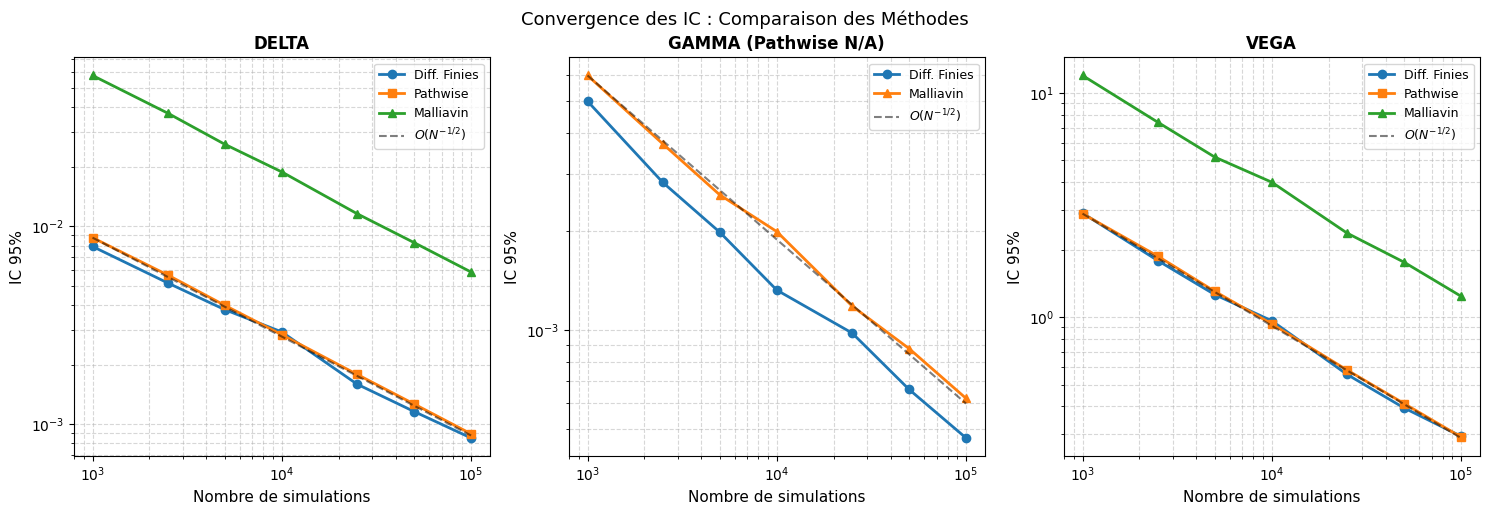
\includegraphics[width=0.95\textwidth]{figures/gamma_comparaison.png}
\caption{Comparaison des méthodes pour le calcul du Gamma. Pathwise est inapplicable (N/A) car $g''(S) = \delta_K$ est une distribution de Dirac.}
\label{fig:gamma}
\end{figure}

\subsubsection{Analyse des Résultats Gamma}

\begin{table}[H]
\centering
\begin{tabular}{lccc}
\toprule
\textbf{Méthode} & \textbf{Estimation} & \textbf{SE} & \textbf{Erreur rel.} \\
\midrule
Black-Scholes (ref.) & \bsGammaFive & -- & -- \\
Différences Finies & \gammaFdEst & \gammaFdSe & \gammaFdErrPct\% \\
Pathwise & \textit{N/A} & -- & -- \\
Malliavin & \gammaMalEst & \gammaMalSe & \gammaMalErrPct\% \\
\bottomrule
\end{tabular}
\caption{Statistiques détaillées pour Gamma ($N = \paramN$). SE = $\sigma_{\text{sample}}/\sqrt{N}$ ; pour FD via bootstrap 200 ré-échantillons.}
\end{table}

\textbf{Observations clés :}
\begin{itemize}
    \item Seules deux méthodes sont applicables pour Gamma
    \item Différences Finies offre une meilleure efficacité (variance plus faible)
    \item Malliavin reste une alternative viable avec variance raisonnable
    \item L'inapplicabilité de Pathwise est une limitation fondamentale pour les Greeks d'ordre 2
\end{itemize}

\subsection{Comparaison pour Vega}

\begin{figure}[H]
\centering
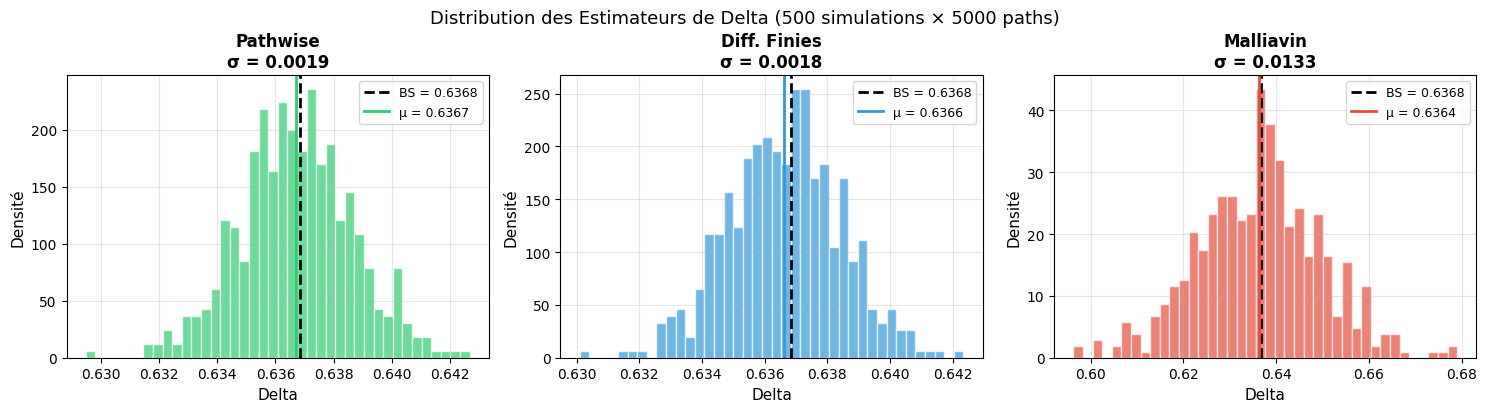
\includegraphics[width=0.95\textwidth]{figures/vega_comparaison.png}
\caption{Comparaison des trois méthodes pour le calcul du Vega.}
\label{fig:vega}
\end{figure}

\subsubsection{Analyse des Résultats Vega}

\begin{table}[H]
\centering
\begin{tabular}{lccc}
\toprule
\textbf{Méthode} & \textbf{Estimation} & \textbf{SE} & \textbf{Erreur rel.} \\
\midrule
Black-Scholes (ref.) & \bsVegaThree & -- & -- \\
Différences Finies & \vegaFdEst & \vegaFdSe & \vegaFdErrPct\% \\
Pathwise & \vegaPwEst & \vegaPwSe & \vegaPwErrPct\% \\
Malliavin & \vegaMalEst & \vegaMalSe & \vegaMalErrPct\% \\
\bottomrule
\end{tabular}
\caption{Statistiques détaillées pour Vega ($N = \paramN$). SE = $\sigma_{\text{sample}}/\sqrt{N}$ ; pour FD via bootstrap 200 ré-échantillons.}
\end{table}

\subsection{Synthèse : Efficacité Relative des Méthodes}

\begin{table}[H]
\centering
\begin{tabular}{l|ccc|c}
\toprule
\textbf{Méthode} & \textbf{Delta} & \textbf{Gamma} & \textbf{Vega} & \textbf{Variance relative} \\
\midrule
Pathwise & \checkmark & $\times$ & \checkmark & $\sim 1\times$ (référence) \\
Différences Finies & \checkmark & \checkmark & \checkmark & $\sim \varRatioFdPw\times$ \\
Malliavin & \checkmark & \checkmark & \checkmark & $\sim \varRatioMalPw\times$ (pire) \\
\bottomrule
\end{tabular}
\caption{Applicabilité et efficacité relative des méthodes (ratio des variances sur Delta, $N = \paramN$).}
\end{table}

% ============================================
\section{Impact de la Discrétisation Temporelle}
% ============================================

\subsection{Motivation}

Pour les options européennes simples sous Black-Scholes, nous pouvons simuler $S_T$ exactement. Cependant, pour les options path-dependent (asiatiques, barrières) ou les modèles plus complexes (volatilité stochastique), nous devons discrétiser la trajectoire.

\subsection{Schéma d'Euler-Maruyama}

\begin{definition}[Schéma d'Euler]
Pour une EDS $dS_t = \mu(S_t) dt + \sigma(S_t) dW_t$, le schéma d'Euler avec $n$ pas de temps est :
$$S_{t_{k+1}} = S_{t_k} + \mu(S_{t_k}) \Delta t + \sigma(S_{t_k}) \Delta W_k$$
où $\Delta t = T/n$ et $\Delta W_k \sim \mathcal{N}(0, \Delta t)$.
\end{definition}

Pour Black-Scholes :
$$S_{t_{k+1}} = S_{t_k} \left( 1 + r \Delta t + \sigma \sqrt{\Delta t} \, Z_k \right)$$

\subsection{Erreur de Discrétisation}

\begin{theoreme}[Convergence du schéma d'Euler]
L'erreur de discrétisation Euler est :
\begin{itemize}
    \item \textbf{Convergence forte} : $\mathbb{E}[|S_T^{\text{Euler}} - S_T^{\text{exact}}|] = O(\sqrt{\Delta t})$
    \item \textbf{Convergence faible} : $|\mathbb{E}[g(S_T^{\text{Euler}})] - \mathbb{E}[g(S_T^{\text{exact}})]| = O(\Delta t)$
\end{itemize}
\end{theoreme}

\subsection{Résultats Numériques}

\begin{figure}[H]
\centering
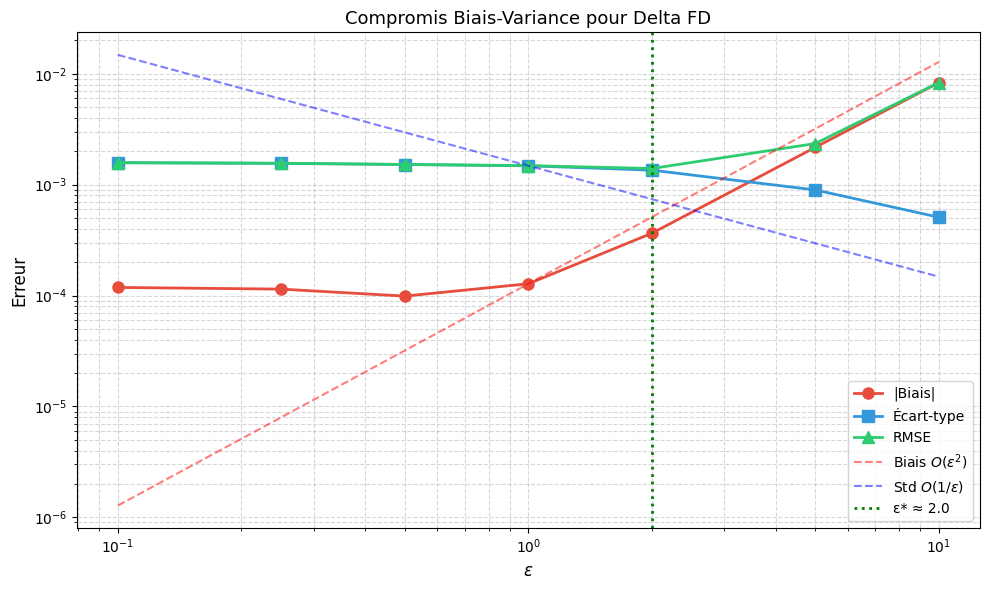
\includegraphics[width=0.95\textwidth]{figures/euler_convergence.png}
\caption{Convergence de l'erreur sur Delta en fonction du nombre de pas Euler. L'erreur décroît conformément à la théorie. Avec $n = 100$ pas, l'erreur est de l'ordre de $10^{-4}$, négligeable par rapport à l'erreur Monte Carlo.}
\label{fig:euler}
\end{figure}

\subsubsection{Analyse}

\begin{table}[H]
\centering
\begin{tabular}{ccc}
\toprule
\textbf{Pas Euler} $n$ & \textbf{Erreur sur Delta} & \textbf{Temps relatif} \\
\midrule
10  & \eulerErrTen          & 1× \\
50  & \eulerErrFifty        & 5× \\
100 & \eulerErrHundred      & 10× \\
500 & \eulerErrFiveHundred  & 50× \\
\bottomrule
\end{tabular}
\caption{Erreur de discrétisation Euler vs simulation exacte ($N = \paramN$, référence = Delta Pathwise sur trajectoire exacte). À $n \geq 50$, l'erreur de discrétisation devient du même ordre que l'erreur Monte Carlo et son évolution avec $n$ est dominée par le bruit MC.}
\end{table}

\textbf{Recommandation :} Pour la plupart des applications, $n = 100$ pas offre un bon compromis précision/coût : l'erreur de discrétisation est alors du même ordre de grandeur que la SE Monte Carlo ($\sim \deltaPwSe$ pour Delta Pathwise), donc pratiquement négligeable. Au-delà, augmenter $n$ ne réduit plus significativement l'erreur (saturée par le bruit MC) mais augmente proportionnellement le coût.

% ============================================
\section{Validation par Approche EDP}
% ============================================

\subsection{L'Équation de Black-Scholes}

Le prix d'une option $V(S,t)$ satisfait l'EDP de Black-Scholes :
$$\frac{\partial V}{\partial t} + \frac{1}{2}\sigma^2 S^2 \frac{\partial^2 V}{\partial S^2} + rS\frac{\partial V}{\partial S} - rV = 0$$

avec condition terminale $V(S,T) = g(S)$ et conditions aux limites appropriées.

\subsection{Discrétisation par Différences Finies}

L'EDP est résolue numériquement par un schéma implicite (Crank-Nicolson) sur une grille $(S_i, t_j)$.

\textbf{Avantages :}
\begin{itemize}
    \item Résultats \textbf{déterministes} (pas de variance)
    \item Calcul \textbf{simultané} du prix et des Greeks
    \item Excellente précision pour les options européennes
\end{itemize}

\subsection{Greeks par EDP}

Les Greeks sont calculés directement à partir de la solution numérique :
\begin{align}
\Delta_{\text{EDP}} &= \frac{V_{i+1,0} - V_{i-1,0}}{S_{i+1} - S_{i-1}} \\
\Gamma_{\text{EDP}} &= \frac{V_{i+1,0} - 2V_{i,0} + V_{i-1,0}}{(\Delta S)^2}
\end{align}

\subsection{Résultats Comparatifs}

\begin{table}[H]
\centering
\begin{tabular}{lccc}
\toprule
\textbf{Quantité} & \textbf{EDP} & \textbf{Black-Scholes} & \textbf{Erreur abs.} \\
\midrule
Prix  & \pdePrice & \bsPrice & \pdeErrPrice \\
Delta & \pdeDelta & \bsDelta & \pdeErrDelta \\
Gamma & \pdeGamma & \bsGamma & \pdeErrGamma \\
Vega  & \pdeVega  & \bsVega  & \pdeErrVega \\
\bottomrule
\end{tabular}
\caption{Validation EDP (Crank-Nicolson, grille $S_{\max}=300$, $N_S=N_t=200$) vs Black-Scholes analytique.}
\end{table}

\textbf{Observations :}
\begin{itemize}
    \item Les erreurs EDP sont très faibles ($< 0.02$ pour Delta, $< 0.001$ pour Gamma)
    \item L'EDP fournit une validation indépendante des méthodes Monte Carlo
    \item La cohérence entre les trois approches (analytique, MC, EDP) renforce la confiance dans les résultats
\end{itemize}

\subsection{Comparaison Monte Carlo vs EDP}

\begin{table}[H]
\centering
\begin{tabular}{p{5cm}p{5cm}}
\toprule
\textbf{Monte Carlo} & \textbf{EDP} \\
\midrule
\begin{itemize}[leftmargin=*]
    \item Stochastique (variance)
    \item Haute dimension possible
    \item Options path-dependent
    \item Convergence $O(N^{-1/2})$
\end{itemize}
&
\begin{itemize}[leftmargin=*]
    \item Déterministe (pas de variance)
    \item Limité à 2-3 dimensions
    \item Options européennes principalement
    \item Convergence $O((\Delta S)^2)$
\end{itemize}
\\
\bottomrule
\end{tabular}
\caption{Comparaison des approches Monte Carlo et EDP}
\end{table}

% ============================================
\section{Conclusion et Recommandations}
% ============================================

\subsection{Synthèse des Résultats}

Ce travail a présenté une étude comparative approfondie de trois méthodes Monte Carlo pour le calcul des Greeks :

\begin{enumerate}
    \item \textbf{Différences Finies (FD)} : Méthode universelle mais présentant un compromis biais-variance sur le choix de $\varepsilon$.
    
    \item \textbf{Pathwise} : Méthode optimale (variance minimale, pas de biais) pour les Greeks d'ordre 1 de payoffs différentiables, mais inapplicable pour Gamma.
    
    \item \textbf{Malliavin (LRM)} : Méthode universelle applicable même aux payoffs discontinus, mais souffrant d'une variance significativement plus élevée.
\end{enumerate}

Les résultats numériques confirment la convergence des trois méthodes vers les valeurs théoriques de Black-Scholes, validant ainsi les implémentations.

\subsection{Recommandations Pratiques}

\begin{table}[H]
\centering
\begin{tabular}{lll}
\toprule
\textbf{Situation} & \textbf{Méthode recommandée} & \textbf{Justification} \\
\midrule
Call/Put européens & Pathwise & Variance minimale \\
Options digitales & Malliavin & Seule applicable \\
Gamma (tous payoffs) & FD ou Malliavin & Pathwise N/A \\
Prototypage rapide & Différences Finies & Simplicité \\
Validation & EDP / analytique & Déterministe \\
\bottomrule
\end{tabular}
\caption{Guide de sélection des méthodes}
\end{table}

\subsubsection{Paramètres Optimaux}

\begin{itemize}
    \item \textbf{Nombre de simulations} : $N \geq 50\,000$ pour IC 95\% raisonnable
    \item \textbf{Pas Euler} : $n \geq 100$ pour erreur de discrétisation négligeable
    \item \textbf{Epsilon (FD)} : $\varepsilon \approx 1$ pour $N = 50\,000$
    \item \textbf{Réduction de variance} : Variables antithétiques systématiquement, CRN pour FD
\end{itemize}

\subsection{Extensions et Perspectives}

Ce travail peut être étendu dans plusieurs directions :

\begin{enumerate}
    \item \textbf{Autres Greeks} : Theta ($\partial V/\partial t$), Rho ($\partial V/\partial r$), Greeks croisés (Vanna, Volga)
    
    \item \textbf{Options exotiques} : Application aux asiatiques, barrières, lookback où Monte Carlo est incontournable
    
    \item \textbf{Modèles avancés} : Volatilité stochastique (Heston), taux stochastiques (Hull-White), modèles à sauts
    
    \item \textbf{Quasi-Monte Carlo} : Utilisation de séquences de Sobol pour améliorer la convergence à $O(N^{-1})$
    
    \item \textbf{Différentiation Automatique} : Utilisation d'outils modernes (JAX, PyTorch) pour automatiser Pathwise
\end{enumerate}

% ============================================
% BIBLIOGRAPHIE
% ============================================
\newpage
\begin{thebibliography}{99}

\bibitem{blackscholes}
Black, F., \& Scholes, M. (1973). The Pricing of Options and Corporate Liabilities. \textit{Journal of Political Economy}, 81(3), 637-654.

\bibitem{glasserman}
Glasserman, P. (2003). \textit{Monte Carlo Methods in Financial Engineering}. Springer.

\bibitem{broadie}
Broadie, M., \& Glasserman, P. (1996). Estimating Security Price Derivatives Using Simulation. \textit{Management Science}, 42(2), 269-285.

\bibitem{fournie}
Fournié, E., Lasry, J.-M., Lebuchoux, J., Lions, P.-L., \& Touzi, N. (1999). Applications of Malliavin Calculus to Monte Carlo Methods in Finance. \textit{Finance and Stochastics}, 3(4), 391-412.

\bibitem{hull}
Hull, J. C. (2017). \textit{Options, Futures, and Other Derivatives} (10th ed.). Pearson.

\bibitem{shreve}
Shreve, S. E. (2004). \textit{Stochastic Calculus for Finance II: Continuous-Time Models}. Springer.

\end{thebibliography}

\end{document}
